\documentclass{article}

\usepackage[top=3cm, bottom=3cm, left=3.5cm,right=3.5cm]{geometry}
\usepackage[colorinlistoftodos]{todonotes}
\usepackage{graphicx}
\usepackage{bm}
\usepackage{titlesec}
\usepackage{amssymb}
\usepackage{amsmath}
\usepackage{natbib} % print author's name and year when citing
\usepackage{bbm}
\usepackage{todonotes}
\usepackage{pdflscape}
\usepackage{caption}
\usepackage{subcaption}
\usepackage[T1]{fontenc}
\usepackage[utf8]{inputenc}
\usepackage{authblk}
\usepackage{pdfpages}
\usepackage{setspace} 
\usepackage{booktabs}
\usepackage{longtable}
\usepackage{float}
\usepackage{tikz}
\usepackage[colorlinks=true,citecolor=blue, linkcolor=blue]{hyperref}
\usepackage{multirow}
\usepackage{todonotes}

\usepackage{tikz}

\setlength{\tabcolsep}{5pt}
%%\setlength{\parindent}{0pt}
\usepackage[parfill]{parskip}
\renewcommand{\arraystretch}{1.5}

\setcounter{tocdepth}{2}

% Define a custom note command for general notes
\newcommand{\mynote}[1]{\todo[color=yellow!40,inline]{#1}}

\DeclareMathOperator*{\argmin}{arg\,min}

% Nature Bibliography style
% \usepackage[backend=biber,style=nature]{biblatex}
% \addbibresource{library.bib} 
\bibliographystyle{unsrtnat}

% number equations by section
\numberwithin{equation}{section}

\title{A clustering framework for conditional extremes models}
\thispagestyle{empty}
\author{Patrick O'Toole, Christian Rohrbeck, Jordan Richards}
\date{\today}

\begin{document}

\maketitle

\todo{Same (present), tense throughout if possible}

% \newpage

\begin{abstract}
  % Intro
 Conditional extreme value models have proven useful for analysing the joint tail behaviour of random vectors. 
 Conditional extreme value models describe the distribution of components of a random vector conditional on at least one exceeding a suitably high threshold, and they can flexibly capture a variety of structures in the distribution tails.
 One drawback of these methods is that model estimates tend to be highly uncertain due to the natural scarcity of extreme data. 
 This motivates the development of clustering methods for this class of models; pooling similar within-cluster data drastically reduces parameter estimation uncertainty.
 
 While an extensive amount of work to estimate conditional extremes models exists in multivariate and spatial applications, the prospect of clustering for models of this type has not yet been explored. 
 As a motivating example, we explore tail dependence of meteorological variables across multiple spatial locations and seek to identify sites which exhibit similar multivariate tail behaviour. 
 To this end, we introduce a clustering framework for conditional extremes models which provides a novel and principled, parametric methodology for summarising multivariate extremal dependence.
 
 % Outline of model
 In a first step, we define a dissimilarity measure for conditional extremes models based on the Jensen-Shannon divergence and common working assumptions made when fitting these models. 
 One key advantage of our measure is that it can be applied in arbitrary dimension and, as opposed to existing methods for clustering extremal dependence, is not restricted to a bivariate setting. 
 Clustering is then performed by applying the k-medoids algorithm to our novel dissimilarity matrix, which collects the dissimilarity between all pairs of spatial sites. 
 
 % Simulation
 A detailed simulation study shows our technique to be superior to the leading competitor in the bivariate case across a range of possible dependence structures and uniquely provides a tool for clustering in the multivariate extremal dependence setting. 
 We also outline a methodology for selecting the number of clusters to use in a given application.  Finally, we apply our clustering framework to meteorological data from Ireland and air pollution data in cities across the US (United States). 

\end{abstract}

\newpage

\tableofcontents

\newpage

\section{Introduction}\label{sec:intro}
\todo{Where to describe Vignotto method? in introduction?}
\todo{Will have to mention that other paper that does bivaraite clustering as well in background, right?}

\section{Motivating examples}
\subsection{Irish meteorological data} \label{subsec:mot_irl}
\todo{Copy mostly from TFR, will have to include NI data}

\begin{itemize}
    \item 
\end{itemize}

\subsection{US urban air pollution} \label{subsec:mot_us}
\todo{See Huser paper for inspiration}

\begin{itemize}
    \item 
\end{itemize}

\section{Methods}
\todo{Or call subsections Marginal and dependence modelling? See other papers on CE}
\subsection{Peaks-over-threshold}
\subsection{Extremal dependence}
\subsection{Conditional extremes}
\subsection{Jensen-Shannon divergence}
\subsection{Clustering}

\section{Simulation study}\label{sec:sim}
\todo{May not be subsections, but will form structure of this section}
\todo{Do I want to add any visualisations of LRI here? Any ideas there?}
\todo{May want tables instead of figures for some/all simulation results}
\todo{How do I get the $\rho$ in ggplot to match the font used in $\LaTeX$? and not clip?}
\todo{Should I smooth across points in sum plots with geomsmooth?}

% \todo{Introduce each section}
% \todo{Change to not all be ``in section 3''}
% \begin{itemize}
%   \item Throughout this section, we evaluate the effectiveness of our clustering method using a simulation study.
%   \item In \ref{subsec:sim_design}, we describe the mixture of normal and t-copulas used to generate the data for our simulated experiments. 
%   \item \ref{subsec:sim_competing_methods} compares our method to the leading competitor in the bivariate case, \cite{Vignotto2021}.
%   % In \item \ref{subsec:sim_extension}, we extend our method to three dimensions, showing how our model can uniquely cluster in the multivariate extremal dependence setting.
%   \item \ref{subsec:sim_extension} shows how our method can be extended to three dimensions, and uniquely cluster in the multivariate extremal dependence setting.
%   \item In \ref{subsec:sim_realistic}, we apply our method to a more realistic example, with the simulation study designed to somewhat mimic the structure of the Irish dataset introduced in \ref{subsec:mot_irl}.
%   \item In \ref{subsec:sim_refit}, we evaluate the uncertainty in parameter estimates pre- and post-clustering using the bootstrapping scheme from \cite{Heffernan2004}.
%   \item Finally, \ref{subsec:sim_n_clust} outlines a methodology for selecting the number of clusters to use in a given application, and show it's effectiveness using our simulated data. \todo{May have to move to methods, do we want results for this?}
% \end{itemize}

% Introduce section
\begin{itemize}
  \item Throughout this section, we evaluate the effectiveness of our clustering method using a simulation study.
  \item In \ref{subsec:sim_gauss}, we describe a simple simulation design using a Gaussian copula to generate data.
  This data has the advantage of having theoretical asymptotic values for the CE model parameters, to which we can directly compare our estimates.
  \item In \ref{subsec:sim_mixture}, we extend this study to a more complex simulation design using a mixture of Gaussian and t-copulas, for a variety of simple and more complex dependence structures and scenarios. 
  We evaluate our clustering solution using the ARI, and ascertain the improvement of parameter estimation post-clustering using a bootstrapping scheme. \todo{Rewrite}
\end{itemize}

\subsection{Gaussian copula} \label{subsec:sim_gauss}

% Single location
Our Gaussian copula simulation design for a single ``location'', nomenclature chosen to match the spatial nature of our applications, is as follows:
\begin{itemize}
  \item We generate multivariate data from a bivariate Gaussian copula, where we control the dependence structure through its correlation parameter, $\rho_{N}$. 
    \cite{Keef2019} show that for a bivariate Gaussian copula, the asymptotic CE parameters are $\alpha = \sign(\rho_{\text{Gauss}} \rho_{\text{Gauss}}^2, \beta = \frac{1}{2}$, indicating extremal independence. \todo{Fix citations}
  \item We sample from this copula and transform to GPD margins with shape $\xi = -0.05$, scale $\sigma = 1$, giving us our variables. \todo{mention why we chose these?}
  \item Each variable in this multivariate dataset may represent, for example, a meteorological or air pollution variable at a given location.
  \item We can then transform the Laplace margins and use the CE model to estimate the multivariate extremal dependence structure at this location.
\end{itemize}

\vspace{1cm}

% Multiple locations
\begin{itemize}
  \item We can easily extend this design by generating multiple locations with the same and different $\rho_{\text{Gauss}}$.
  \item The knowledge of these parameters provides our ``known'' clustering solution.
  \item For example, we could generate data for four locations, two of which have $\rho_{\text{Gauss}} = 0.1$, and the other two have $\rho_{\text{Gauss}} = 0.9$. 
  \item We can use the CE model to estimate the multivariate extremal dependence structure at each location, and then apply the JS divergence to cluster these locations based on the similarity of the estimated CE parameters. 
  \item These simulations can be repeated many times and we can evaluate the clustering solution using the ARI, and evaluate the bias and variance of our estimates around their theoretical values.
\end{itemize}

% results
\begin{itemize}
  \item To this end, we generated data for 12 locations each with 1000 observations of two variables using the above design.
  \item Three known clusters were designated by having $\rho_{\text{Gauss}}$ values of 0.1, 0.5, and 0.9 respectively for four locations each.
  \item Conditional dependence quantiles of 0.9 and 0.99 were used to estimate the CE model parameters before and after clustering. 
  \item The number of clusters $k$ was ascertained using the method described in ? \todo{reference part of methods that describes this}
  \item Simulations were repeated 500 times, and the results are plotted in figure \ref{fig:00_gauss_cop}.
  \item The estimation of $k$ and the ARI for this simple example were perfect across all simulations.
  \item Several interesting points can be made from this simulation study.
  \item Pre-clustering, the CE model estimates are more uncertain, especially for $\beta$, where the bias is also larger.
  \item This is especially the case for the higher dependence quantile, where data is scarcer, although this also corresponds to less bias, as we take our data from further into the tail. 
  \item Bias and variance are lower for higher $\rho_{\text{Gauss}}$, which appears to be associated with better convergence to the theoretical asymptotic values.
  \item Post-clustering, the same patterns emerge, but the variability in the estimates is reduced, as desired. \todo{Quote any specific values?}
\end{itemize}

\todo{Stop alpha and beta facet labels from clipping}
\begin{figure}[H]
    \centering
    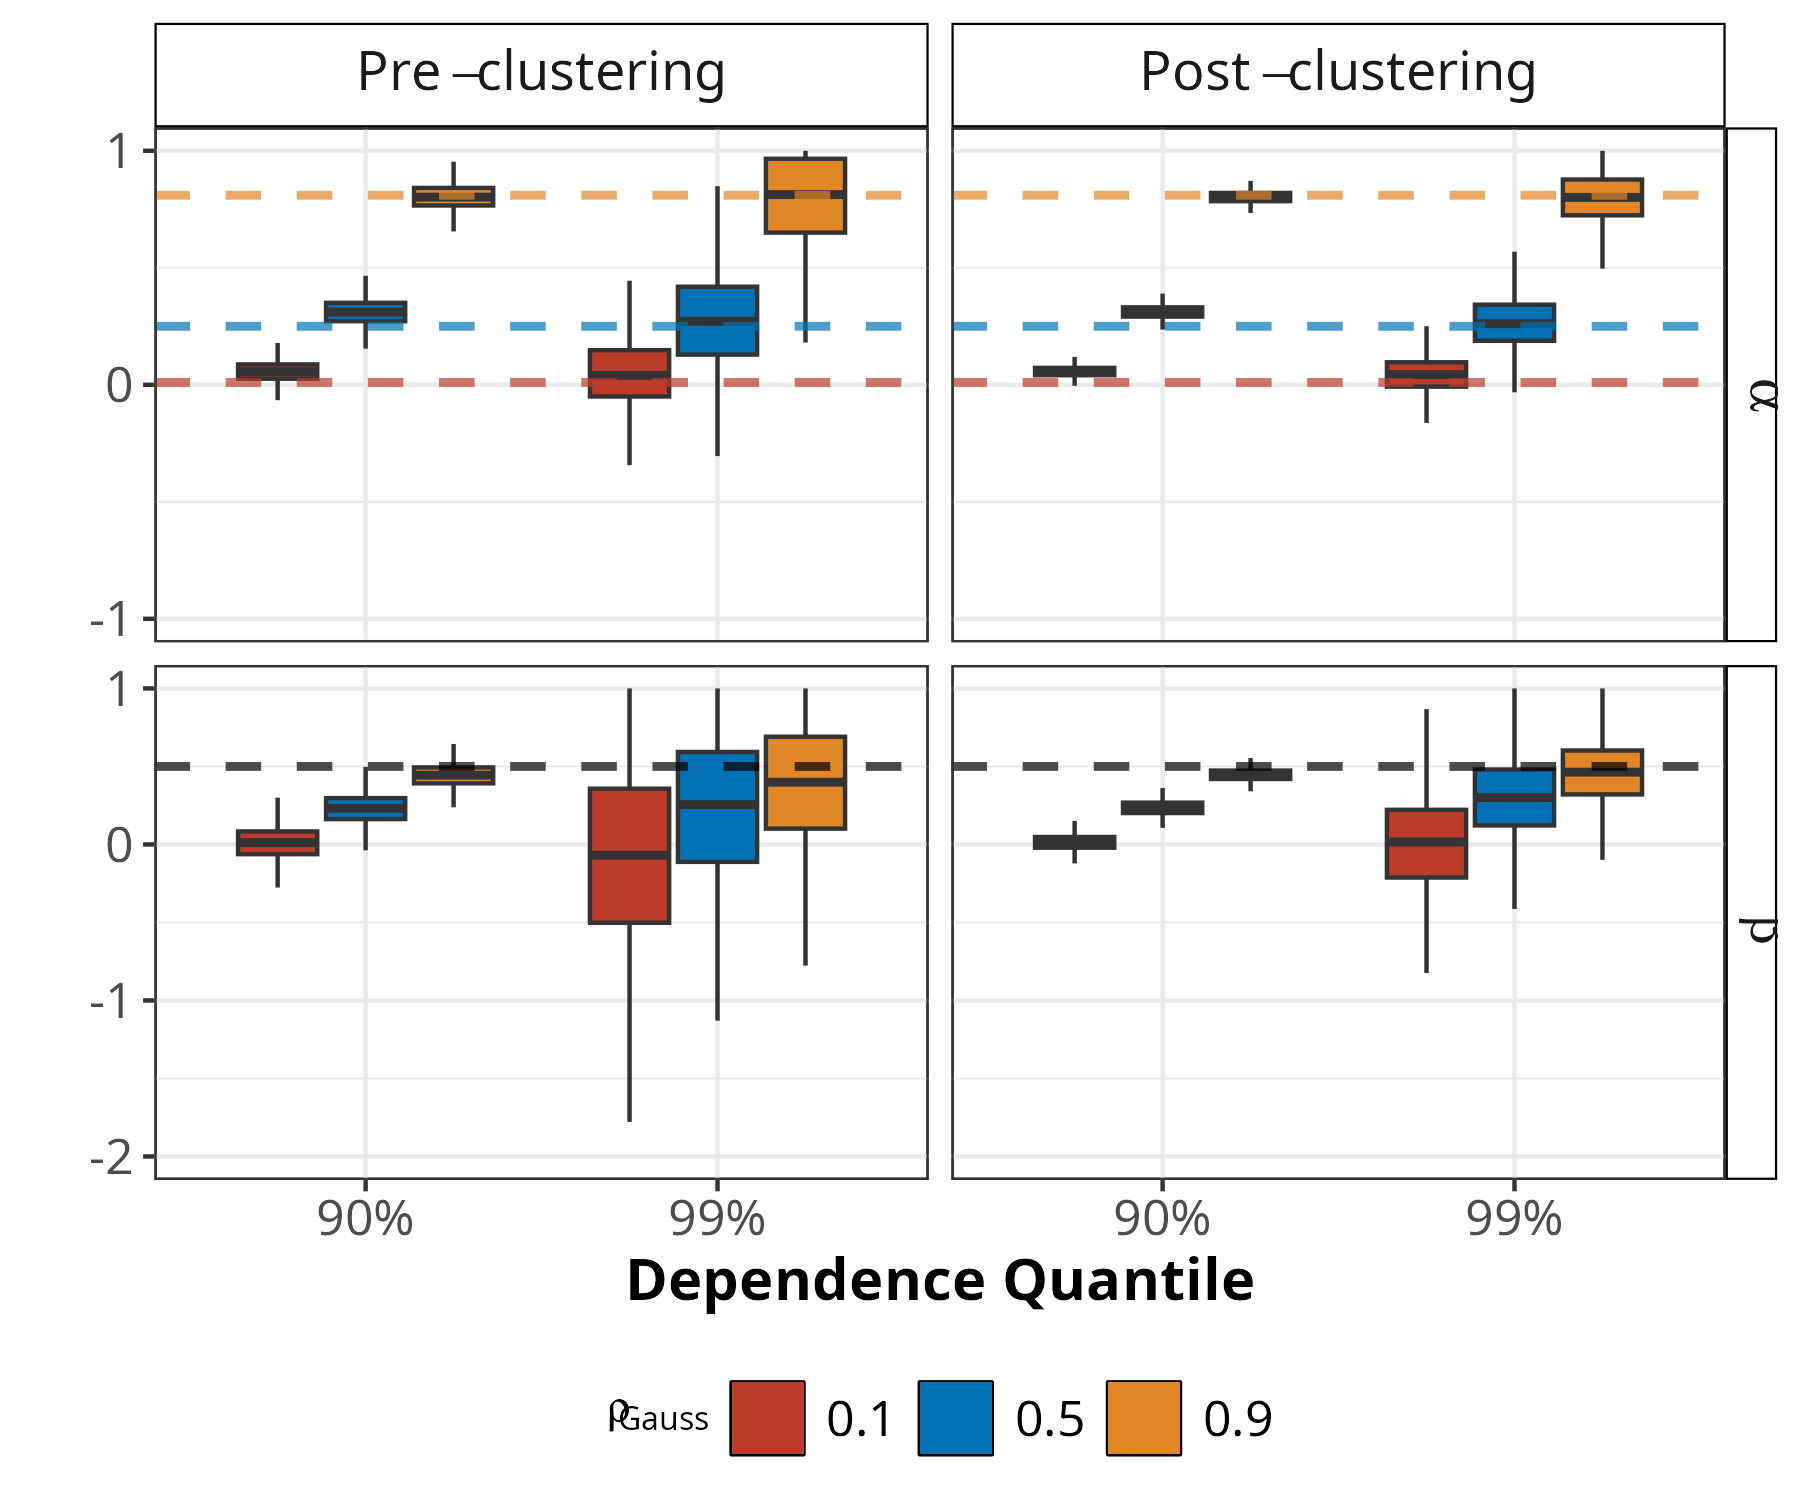
\includegraphics[width = 0.9\linewidth]{plots/sim_01_gauss_cop.png}
    \caption{Boxplots of \emph{$\alpha$ and $\beta$ parameter estimates for the conditional extremes model pre- and post-clustering for a Gaussian copula simulation of 12 datasets, or ``locations'' belonging equally to three known clusters. Simulations were repeated 500 times. The x-axis represents the conditional quantile used to fit the conditional extremes model, and the boxes are coloured by their Gaussian copula correlation parameter, $\rho_{\text{Gauss}}$. Dotted horizontal lines indicate the theoretical asymptotic values of $\alpha$ and $\beta$ for a bivariate Gaussian copula, coloured by the same $\rho_{\text{Gauss}}$ values for $\alpha$ and black for $\beta$ to indicate the same value across all clusters, at $1/2$.}}
    \label{fig:00_gauss_cop}
\end{figure}


\subsection{Mixture models} \label{subsec:sim_mixture}

\begin{itemize}
  \item In this section, we extend our simulation design to a mixture of Gaussian and t-copulas, where we control the dependence structure through their respective correlation parameters, $\rho_{\text{Gauss}}$ and $\rho_{t}$, with each t-copula having 3 degrees of freedom.
  \item The idea behind this design is that the Gaussian copula generates observations exhibiting extremal independence, whereas the t-copula induces extremal dependence, the strength of which is determined by their respective correlation parameters.
  \item While there are no theoretical guarantees about our estimates, we can still evaluate our clustering solution using the ARI.
  \item We can also evaluate the improvement in parameter estimation post-clustering using the bootstrapping scheme described in \cite{Heffernan2004}.
  \item Below, we will describe the results of this simulation study in a variety of scenarios.
\end{itemize}

\subsubsection{Comparison to competing methods} \label{subsubsec:sim_competing_methods}

\todo{Say that we used the max risk function in Vignotto}

% \begin{itemize}
%     \item Compared to method from \cite{Vignotto2021} for two dimensions. 
%     \item Compared using Adjusted Rand Index (ARI) (\todo{cite!}), which compares a clustering solution
%     \item Shown to be an improvement over this method for the overwhelming majority of simulations. 
%     \item \todo{Make interesting comments about how clustering performs better when Gaussian copula correlation is higher!}
% \end{itemize}

\begin{itemize}
  \item We compared our method to the leading competitor in the bivariate case, \cite{Vignotto2021}, using the maximum risk function.
  \item As in \ref{subsec:sim_gauss}, for 500 simulations we generated data for 12 locations each with 1000 observations of two variables, but this time using a mixture of Gaussian and t-copulas with GPD margins. \todo{Extend to 500 simulations, only ran 200 times\!}
  \item Two known clusters were defined using different values of $\rho_t$, keeping $\rho_{\text{Gauss}}$ the same for both (but varying across simulations).
  \item The CE model was fit at the 90th dependence quantile. 
  \item The clustering solutions were evaluated using the ARI, and the results are plotted in figure \ref{fig:01_ce_vs_vi}.
  \item The proposed method is shown to be superior to the leading competitor in the bivariate case, \cite{Vignotto2021}, across a range of possible dependence structures.
  \item Both models perform better when the difference in the t-copula correlation parameters between the two clusters is larger.
  \item Both models also perform better when Gaussian and t-copula correlation are higher, as the signal of extremal dependence is stronger. 
\end{itemize}

\begin{figure}[H]
    \centering
    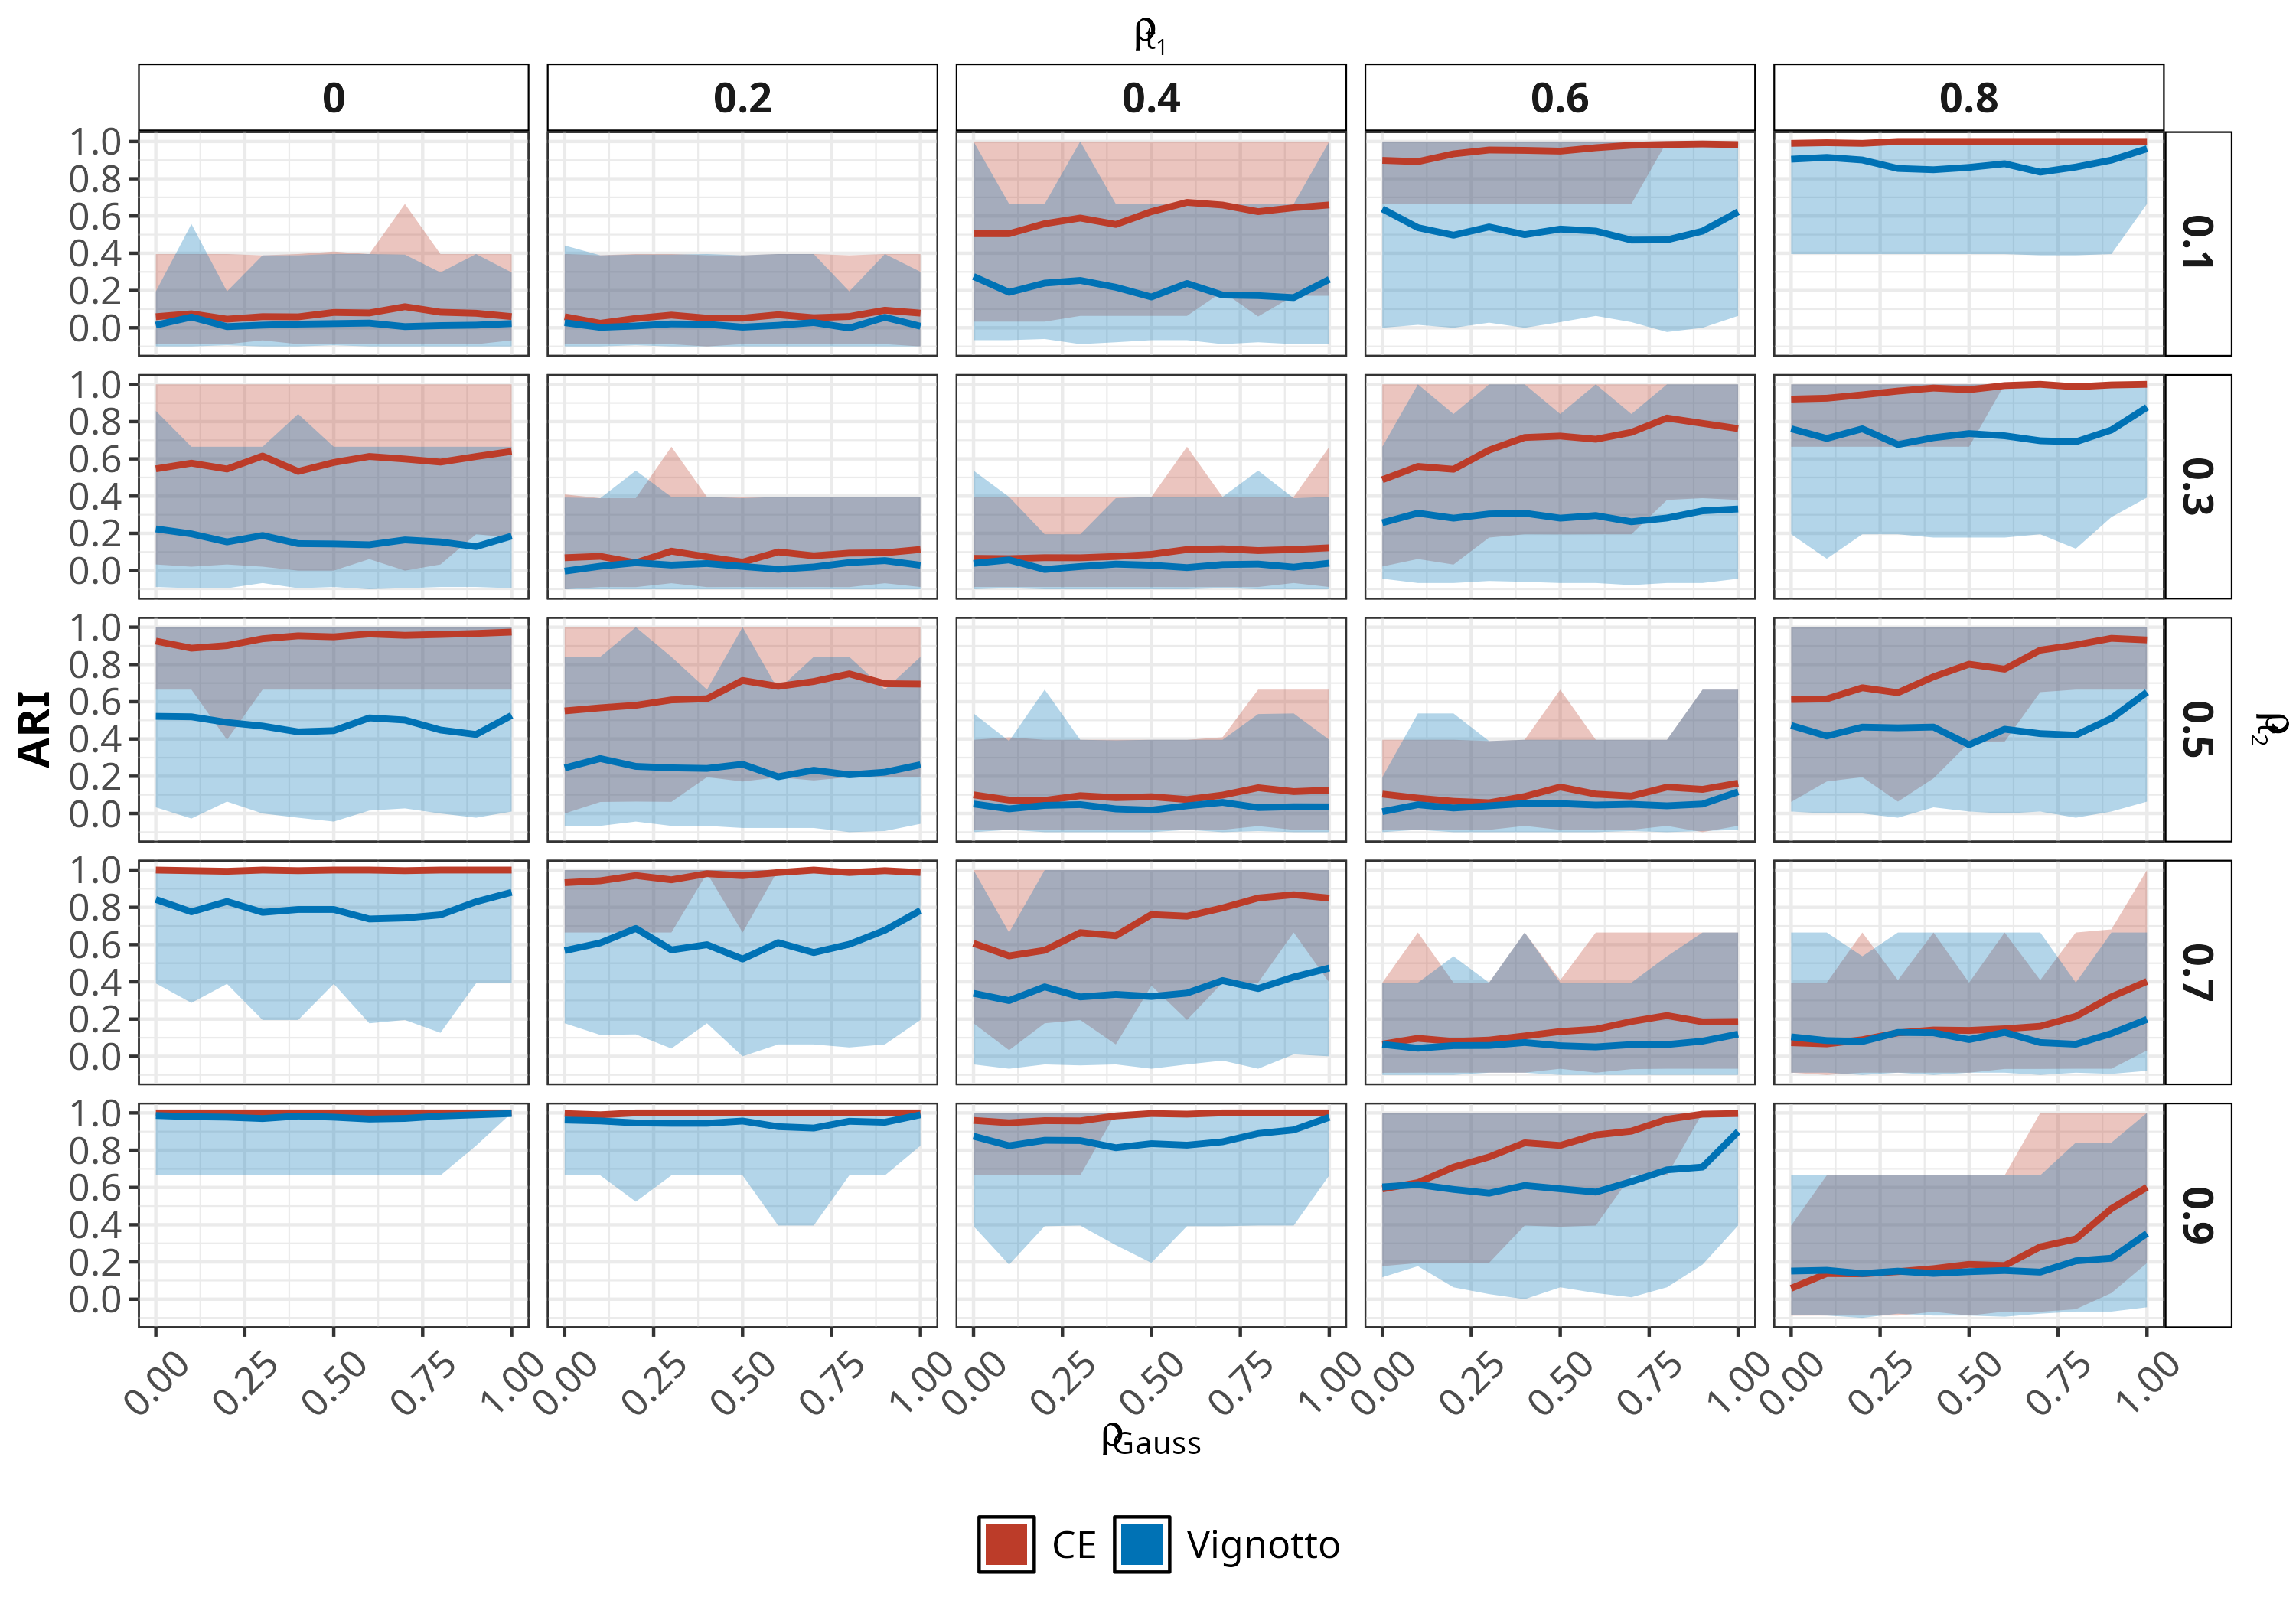
\includegraphics[width = 0.9\linewidth]{plots/sim_01b_ce_vs_vi_dqu_0.9.png}
    \caption{\emph{Comparison of clustering methods for two variables and two equally sized clusters for simulations of 12 ``locations'' from a mixture of Normal and Gaussian copulas. A grid search was performed,  with the x-axis representing the Gaussian correlation parameter used for both clusters, and the facet labels showing the t-copula correlation parameters for each ``known'' cluster. This grid search was repeated 500 times. The lines show the median of the Adjusted Rand Index for both clustering methods, with uncertainty coming from the 90\% credible interval.}} % The proposed method is shown to be superior to the leading competitor in the bivariate case, that of \cite{Vignotto2021}. Both models perform better when the difference in the t-copula correlation parameters between the two clusters is larger, and when Gaussian correlation is higher.}}
    \label{fig:01_ce_vs_vi}
\end{figure}


\subsubsection{Extension to $>2$ dimensions} \label{subsubsec:sim_extension}

% \begin{itemize}
%     \item Also shown to work well for three dimensions ...
% \end{itemize}

\begin{itemize}
  \item While the \cite{Vignotto2021} method is restricted to two dimensions, our method can be extended to three dimensions and beyond.
  \item To illustrate this, we can repeat this simulation study, but with three variables. 
  \item The results are plotted in figure \ref{fig:02_3d}.
  \item The proposed method is shown to work well for three dimensions, and the same patterns emerge as in the bivariate case.
  \item The method is shown to actually perform better in three dimensions than in two.
  \item This comes with the caveat that the variables all have the same GPD marginal distribution, and so including three variables naturally increases the amount of data available to estimate the same dependence structure as in the bivariate case. 
\end{itemize}

\begin{figure}[H]
    \centering
    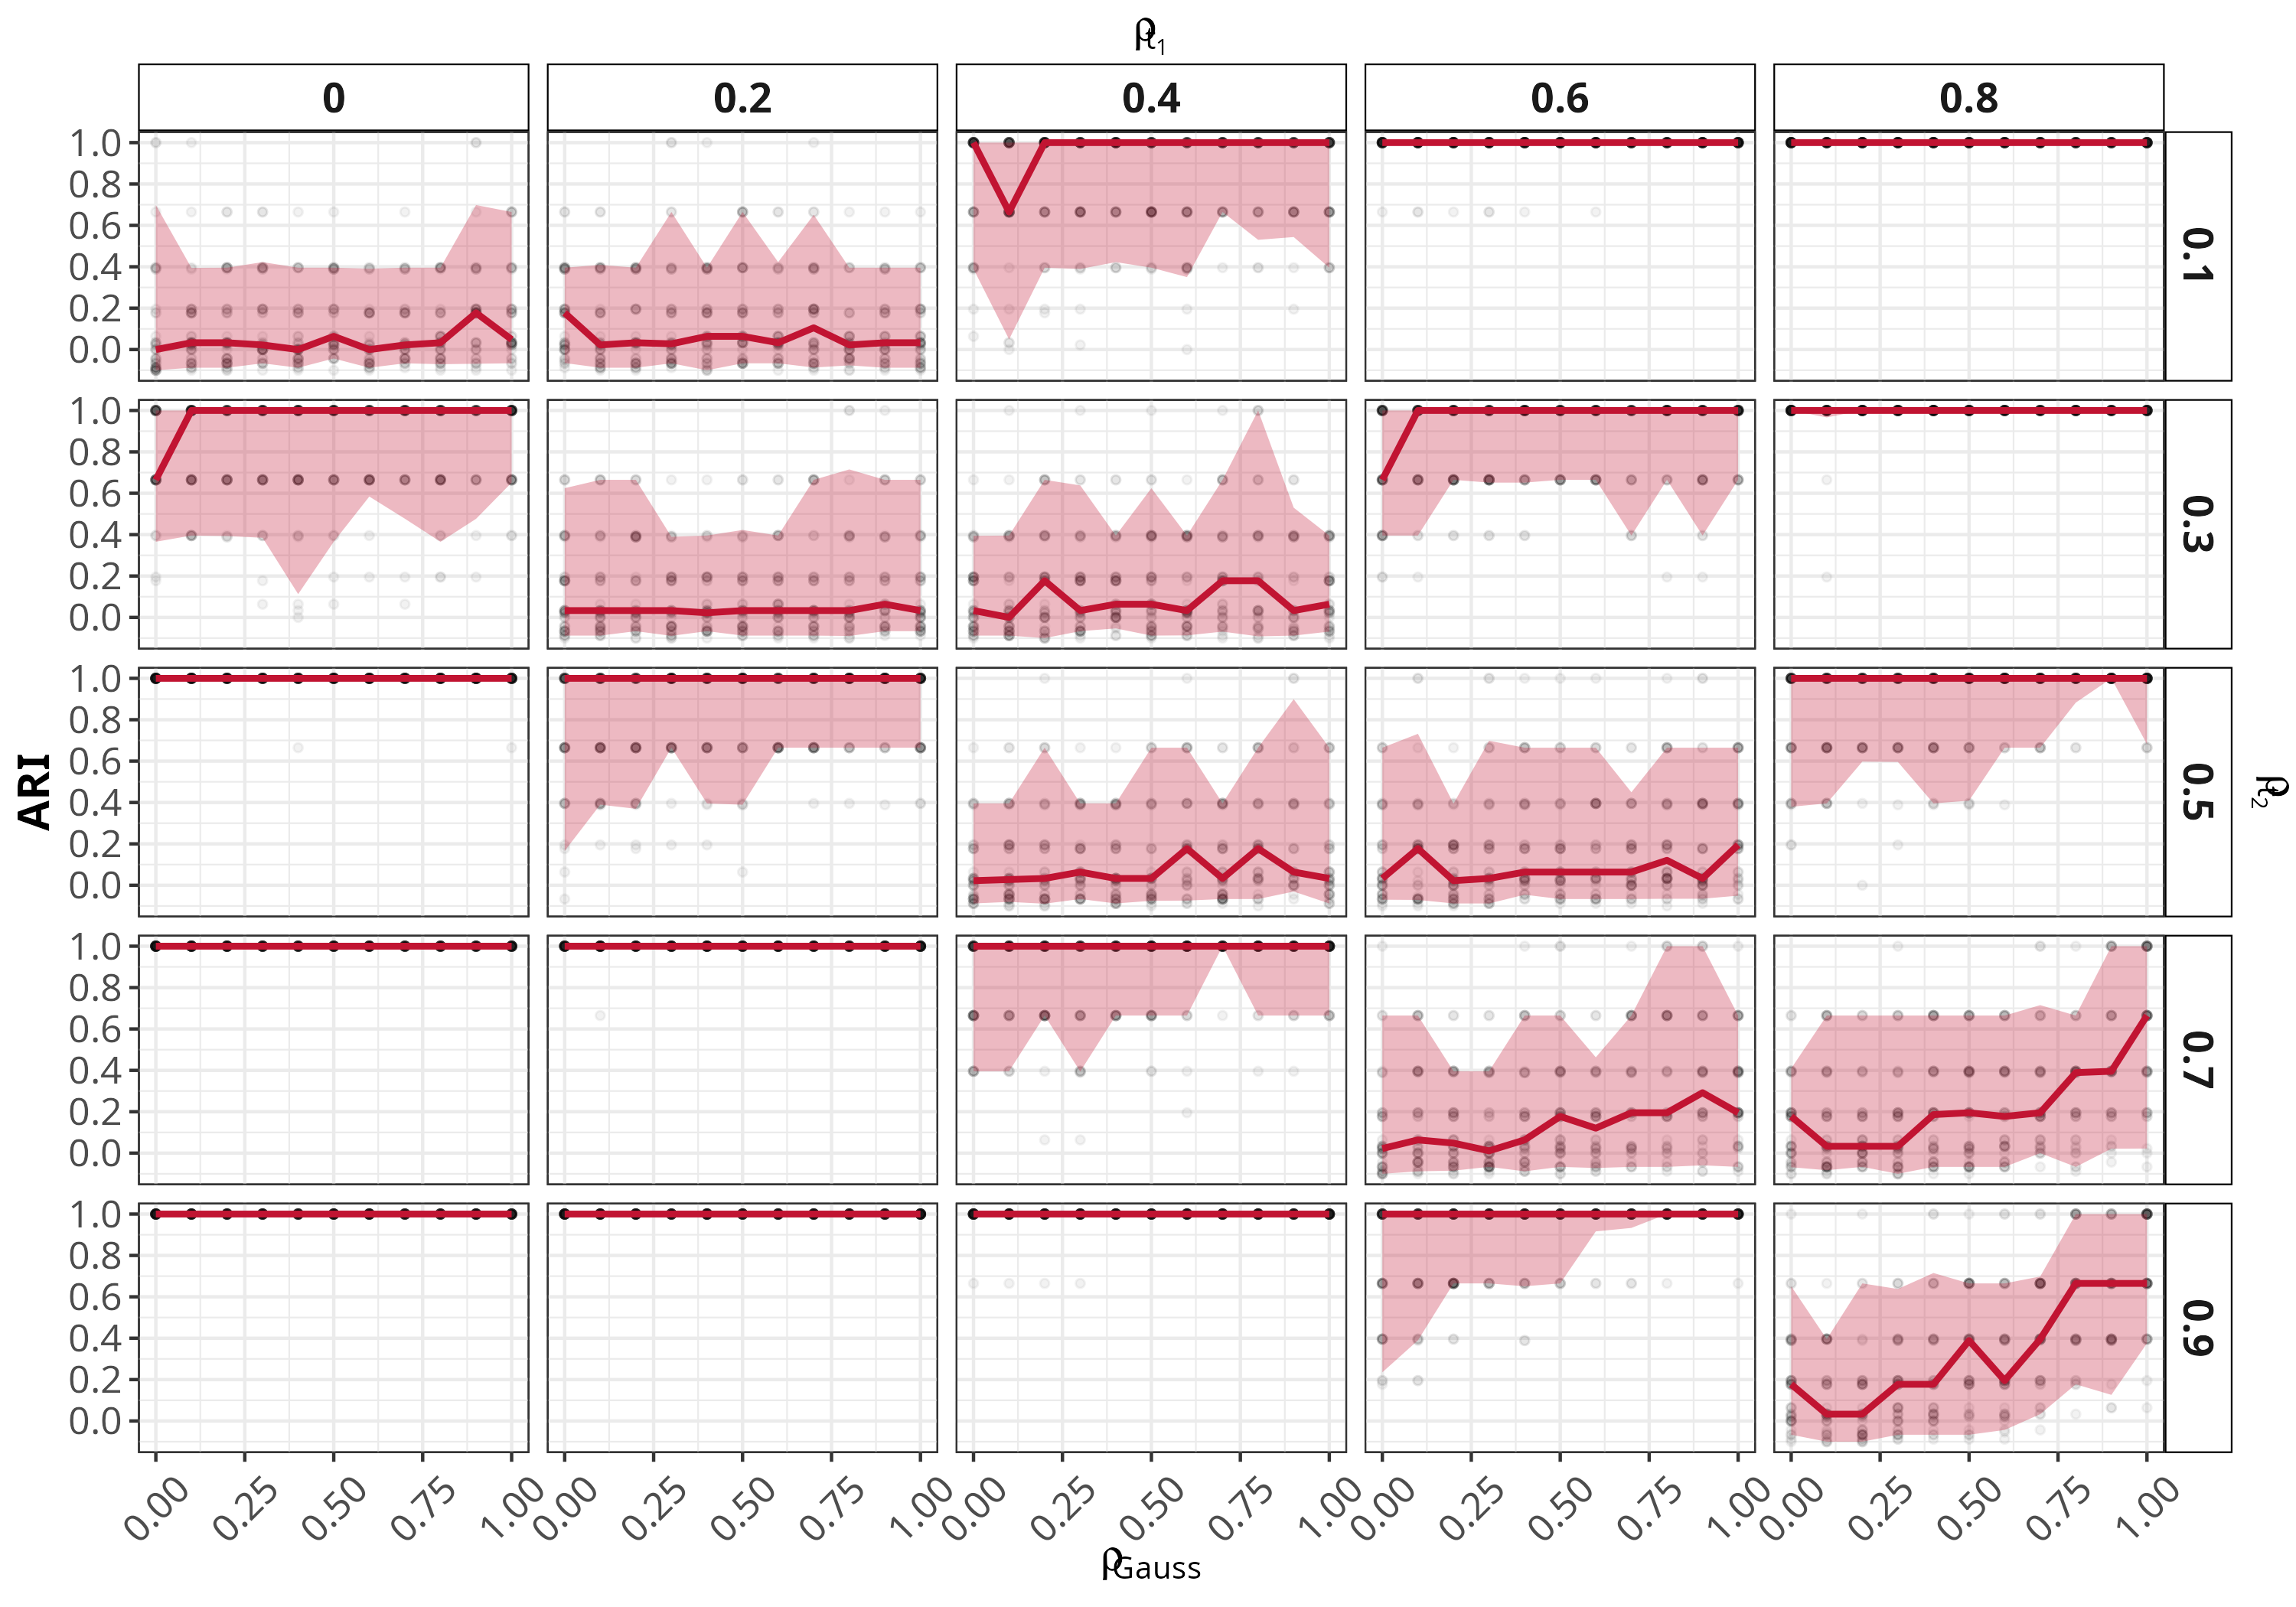
\includegraphics[width = 0.9\linewidth]{plots/sim_01c_js_sens_3_var_dqu_0.9.png}
    \caption{\emph{Evaluation of clustering performance for three variables and two equally sized clusters for simulations of 12 ``locations'' from a mixture of Normal and Gaussian copulas. A grid search was performed,  with the x-axis representing the Gaussian correlation parameter used for both clusters, and the facet labels showing the t-copula correlation parameters for each ``known'' cluster. This grid search was repeated 500 times. The lines show the median of the Adjusted Rand Index for both clustering methods, with uncertainty coming from the 90\% credible interval. Points show individual values of the ARI for a given simulation.}} 
    \label{fig:02_3d}
\end{figure}

\subsubsection{More realistic example} \label{subsubsec:sim_realistic}

% \begin{itemize}
%     \item Generated more realistic example to somewhat match the structure of the Irish dataset. 
%     \item ? locations, ... \todo{fill in}
% \end{itemize}

\begin{itemize}
  \item We generated a more realistic example to somewhat mimic the structure of the Irish dataset introduced in \ref{subsec:mot_irl}.
  \item We generated data from 60 locations, each with 1000 observations of two variables, using a mixture of Gaussian and t-copulas with GPD margins.
  \item The 60 locations had three known clusters, with 30, 20, and 10 locations in each cluster respectively.
  \item A slight perturbation via a uniform sample between $-0.05$ and $0.05$ was added to the correlation parameters of the t-copula for each location, to make the clustering solution more challenging.
  \item Again, clustering was done on the CE model parameters using the JS divergence, the results of which are shown in figure \ref{fig:03_realistic}.
  \item The algorithm is again shown to perform well, particularly where the difference in the t-copula correlation parameters between the clusters is largest. 
\end{itemize}

\todo{Check facet and x-axis labels}
\begin{figure}[H]
    \centering
    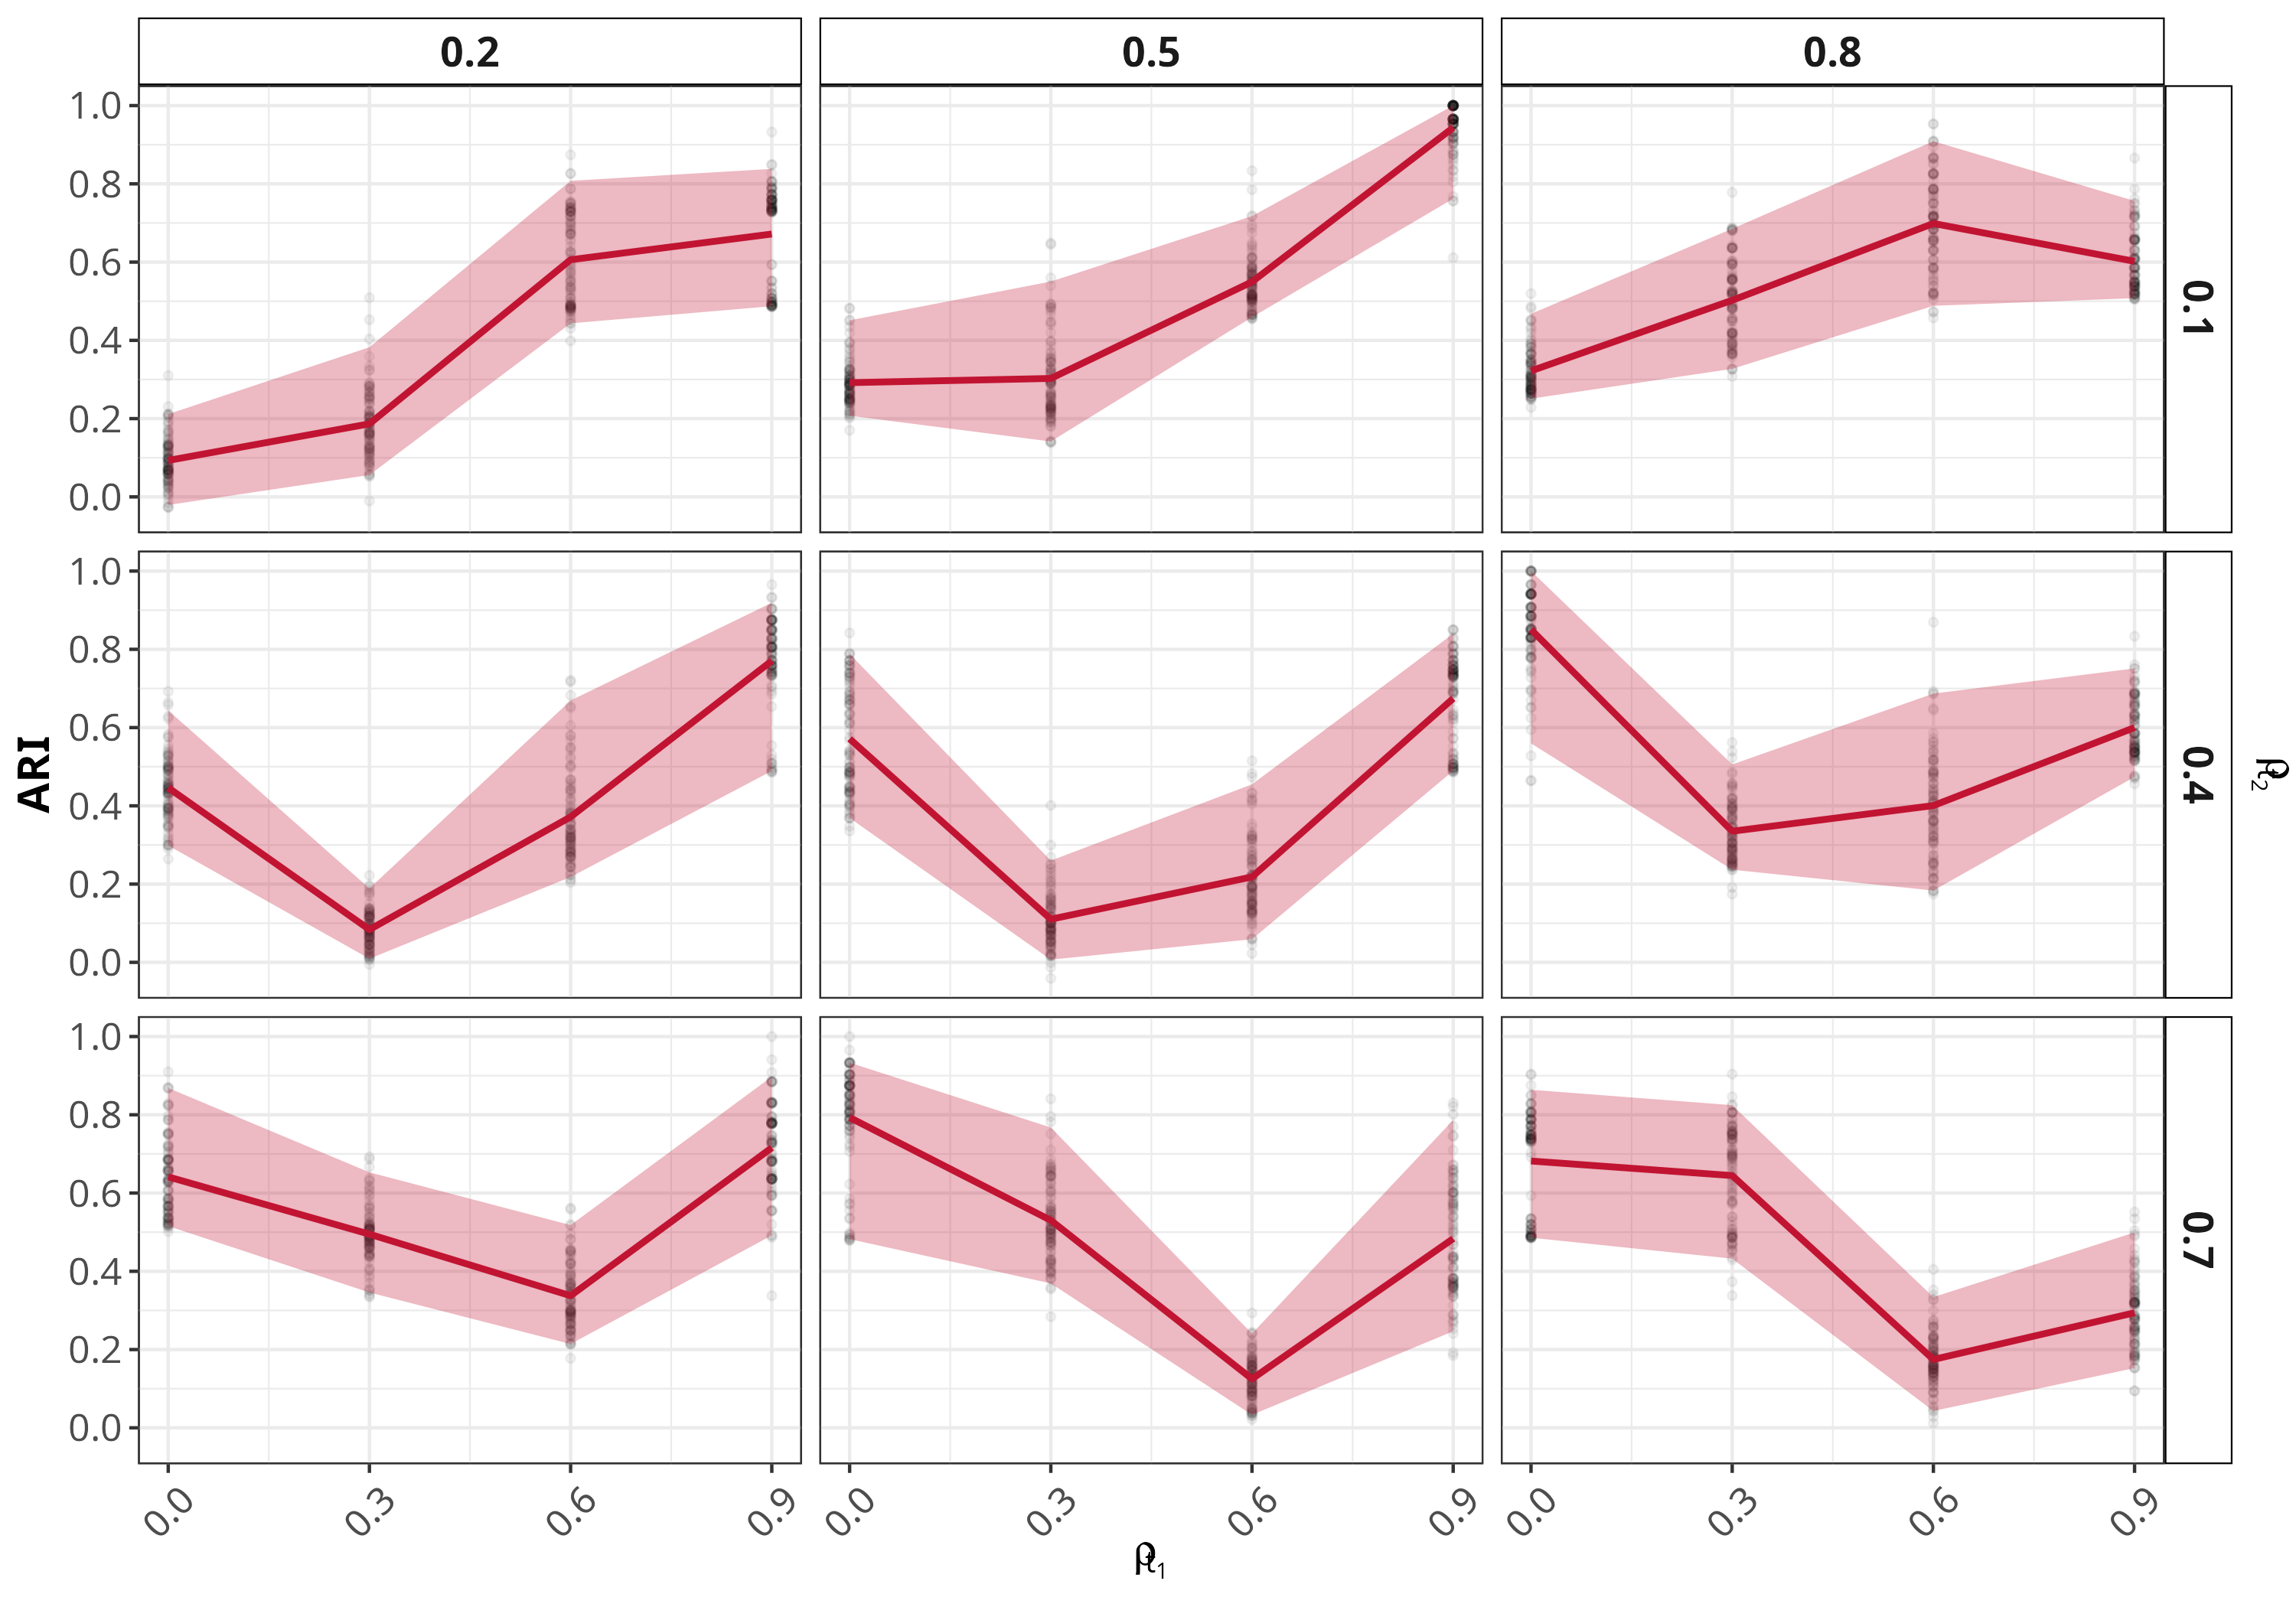
\includegraphics[width = 0.9\linewidth]{plots/sim_01d_js_sens_3_var_dqu_0.9.png}
    \caption{\emph{Evaluation of clustering performance for two variables and three clusters for simulations from a mixture of Normal and Gaussian copulas. 60 locations were simulated with 10, 20 and 30 belonging to each respective cluster. A grid search was performed,  with the x-axis and facet labels showing the t-copula correlation parameters for each of the three ``known'' clusters, for a Gaussian copula correlation of 0.5. Perturbations were added to these parameters. This grid search was repeated 500 times. The line shows the median of the Adjusted Rand Index for both clustering methods, with uncertainty coming from the 90\% credible interval. Points show individual values of the ARI for a given simulation.}} 
    \label{fig:03_realistic}
\end{figure}

\subsubsection{Parameter estimation pre- and post-clustering} \label{subsubsec:sim_refit}

% \begin{itemize}
%     \item Desire to ascertain whether dependence parameters are less uncertain after clustering. 
%     \item Can bootstrap using scheme in \cite{Heffernan2004} to determine uncertainty in parameter estimates. 
%     \item Post clustering, can see that uncertainty is vastly reduced for both $\alpha$ and $\beta$ parameters in this simulation study. 
% \end{itemize}

% Describe bootstrapping
\begin{itemize}
  \item Finally, we recall that a reason for clustering might be to reduce the uncertainty in parameter estimates by grouping similar data together.
  \item To this end, we desired to ascertain whether the estimates of our dependence parameters were less uncertain after clustering.
  \item We can bootstrap using the scheme described in \cite{Heffernan2004} to determine the uncertainty in our parameter estimates. \todo{Describe scheme, how it preserves the dependence structure of the data?}
  \item As we are estimating two parameters, $\alpha$ and $\beta$, for which we do not know the true values, it may be that although our uncertainty is diminished post-clustering, the estimates may still be biased, with the parameters unidentifiable.
  \item There are also many possible combinations of $\alpha$ and $\beta$ that could give the same conditional estimates, and so the estimates may be biased in this sense as well.
  \item To avoid this, we adopt the approach of \cite{Richards2021-qm} in calculating the conditional expectation of one variable given the other is at the $98\%$ marginal quantile $u$, given by
  \begin{equation} \label{eq:boot}
    \mathbb{E}[X_1 | X_2 = u] = \hat{\alpha} u + u^{\hat{\beta}} \hat{\mu},
  \end{equation}
  where ($\hat{\alpha}, \hat{\beta}, \hat{\mu}$) are the estimated CE model parameters.
  \item We can bootstrap this conditional expectation to quantify the reduction in uncertainty post-clustering. \todo{Tense consistency}
\end{itemize}

% Results
\begin{itemize}
  \item We take an example for which we know the clustering algorithm performs well, namely the same simulation design as in \ref{subsubsec:sim_competing_methods}, with $\rho_{\text{Gauss}} = 0.5$, and $\rho_{t} = 0.1$ and $0.9$ for the two clusters.
  \item We estimate the CE model parameters pre- and post-clustering, and bootstrap the conditional expectation of one variable given the other is at the $98\%$ marginal quantile using equation \ref{eq:boot}.
  \item The results are plotted in figure \ref{fig:04_bootstrap}.
  \item We can see that the uncertainty in the bootstrapped estimates is vastly reduced post-clustering, as desired.
  \item The conditional expectation is higher for the higher t-copula correlation cluster, as expected.

\end{itemize}

\todo{Stop clipping for x-axis title}
\begin{figure}[H]
    \centering
    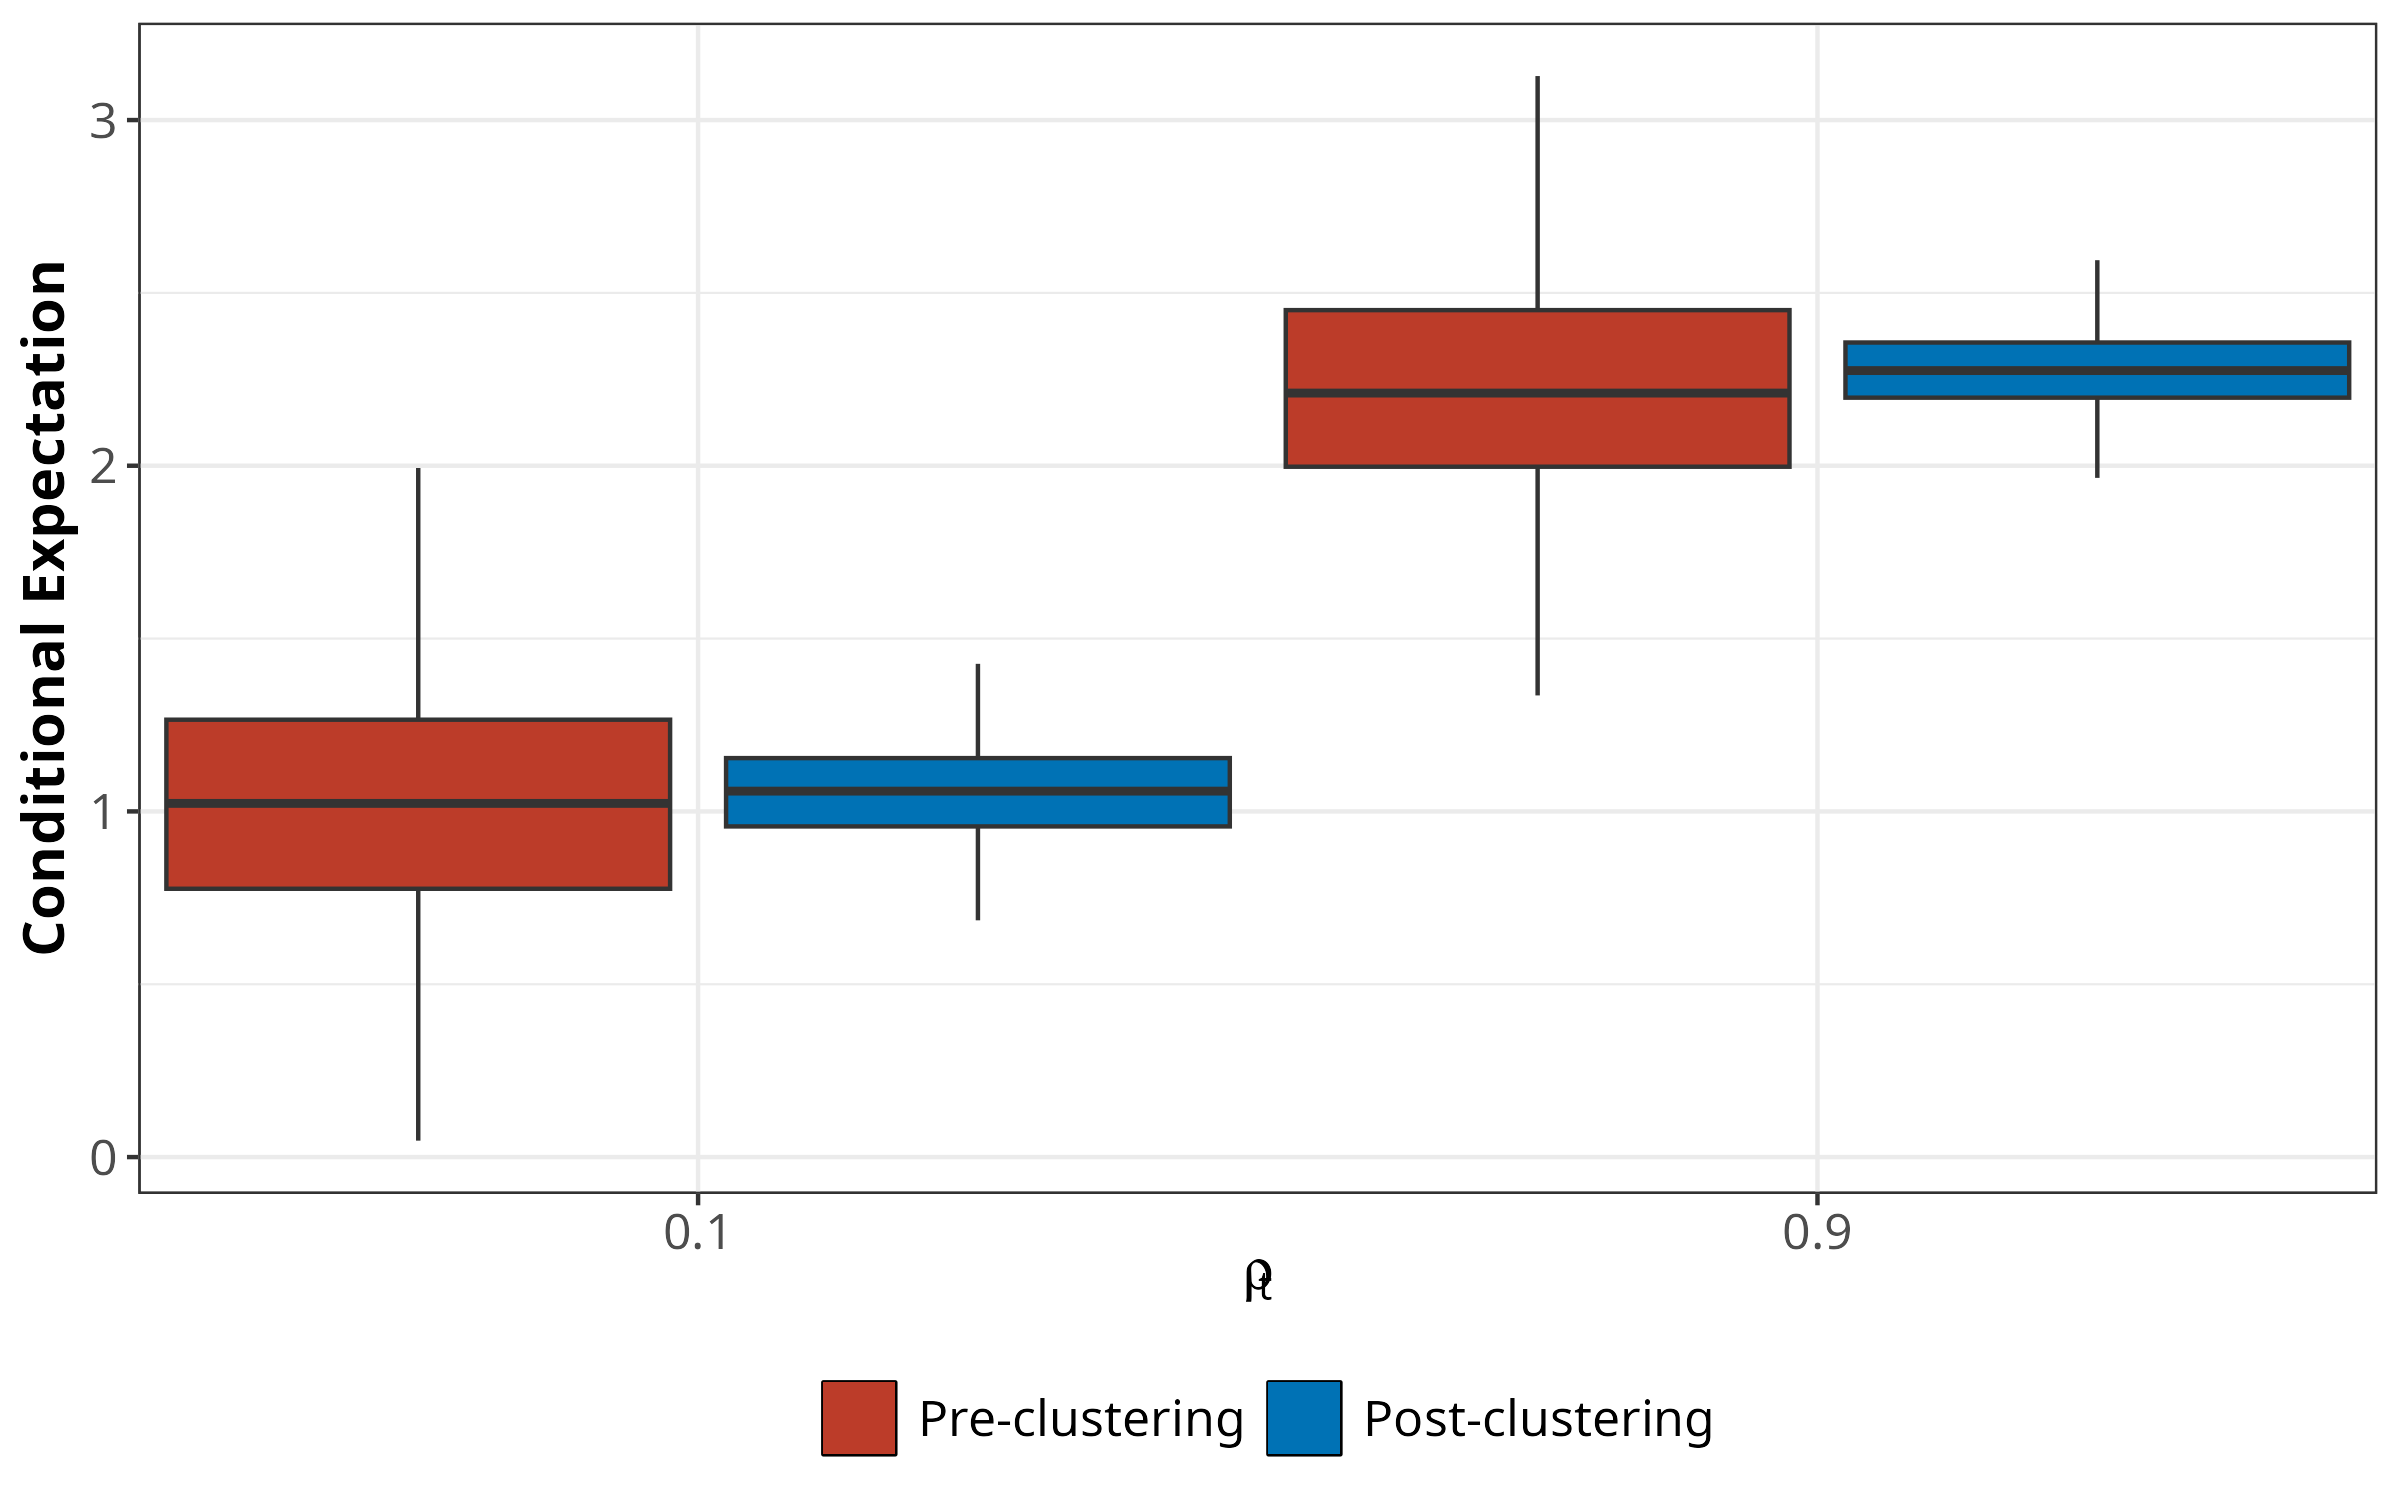
\includegraphics[width = 0.9\linewidth]{plots/sim_01e_bootstrap_box.png}
    \caption{\emph{Boxplots of 500 bootstrapped conditional expectations of one variable given the other is at the $98\%$ marginal quantile $u$, pre- and post-clustering for a simulation of 12 ``locations'' from a mixture of Normal and Gaussian copulas, with the Gaussian correlation set to 0.5. The t-copula correlation parameters for the two clusters were set to 0.1 and 0.9, as shown on the x-axis.}}
    \label{fig:04_bootstrap}
\end{figure}


\section{Applications}
\subsection{Irish meteorological data} \label{subsec:app_irl}

\begin{itemize}
    \item 
\end{itemize}

\subsection{US urban air pollution data} \label{subsec:app_us}

\begin{itemize}
    \item 
\end{itemize}

\section{Discussion}

% Limitations
\begin{itemize}
  \item For simulations, could have looked at LRI as well as ARI.
  \item Could have looked at spatially varying clustering parameters, to more closely mimic spatial applications. 
\end{itemize}

\section*{Code availability}

\newpage
\bibliography{library}

\end{document}
